\begin{column}{\onecolwid} % The third column

%----------------------------------------------------------------------------------------
%	CONCLUSION
%----------------------------------------------------------------------------------------

\begin{block}{Classifier comparison}
\begin{figure}
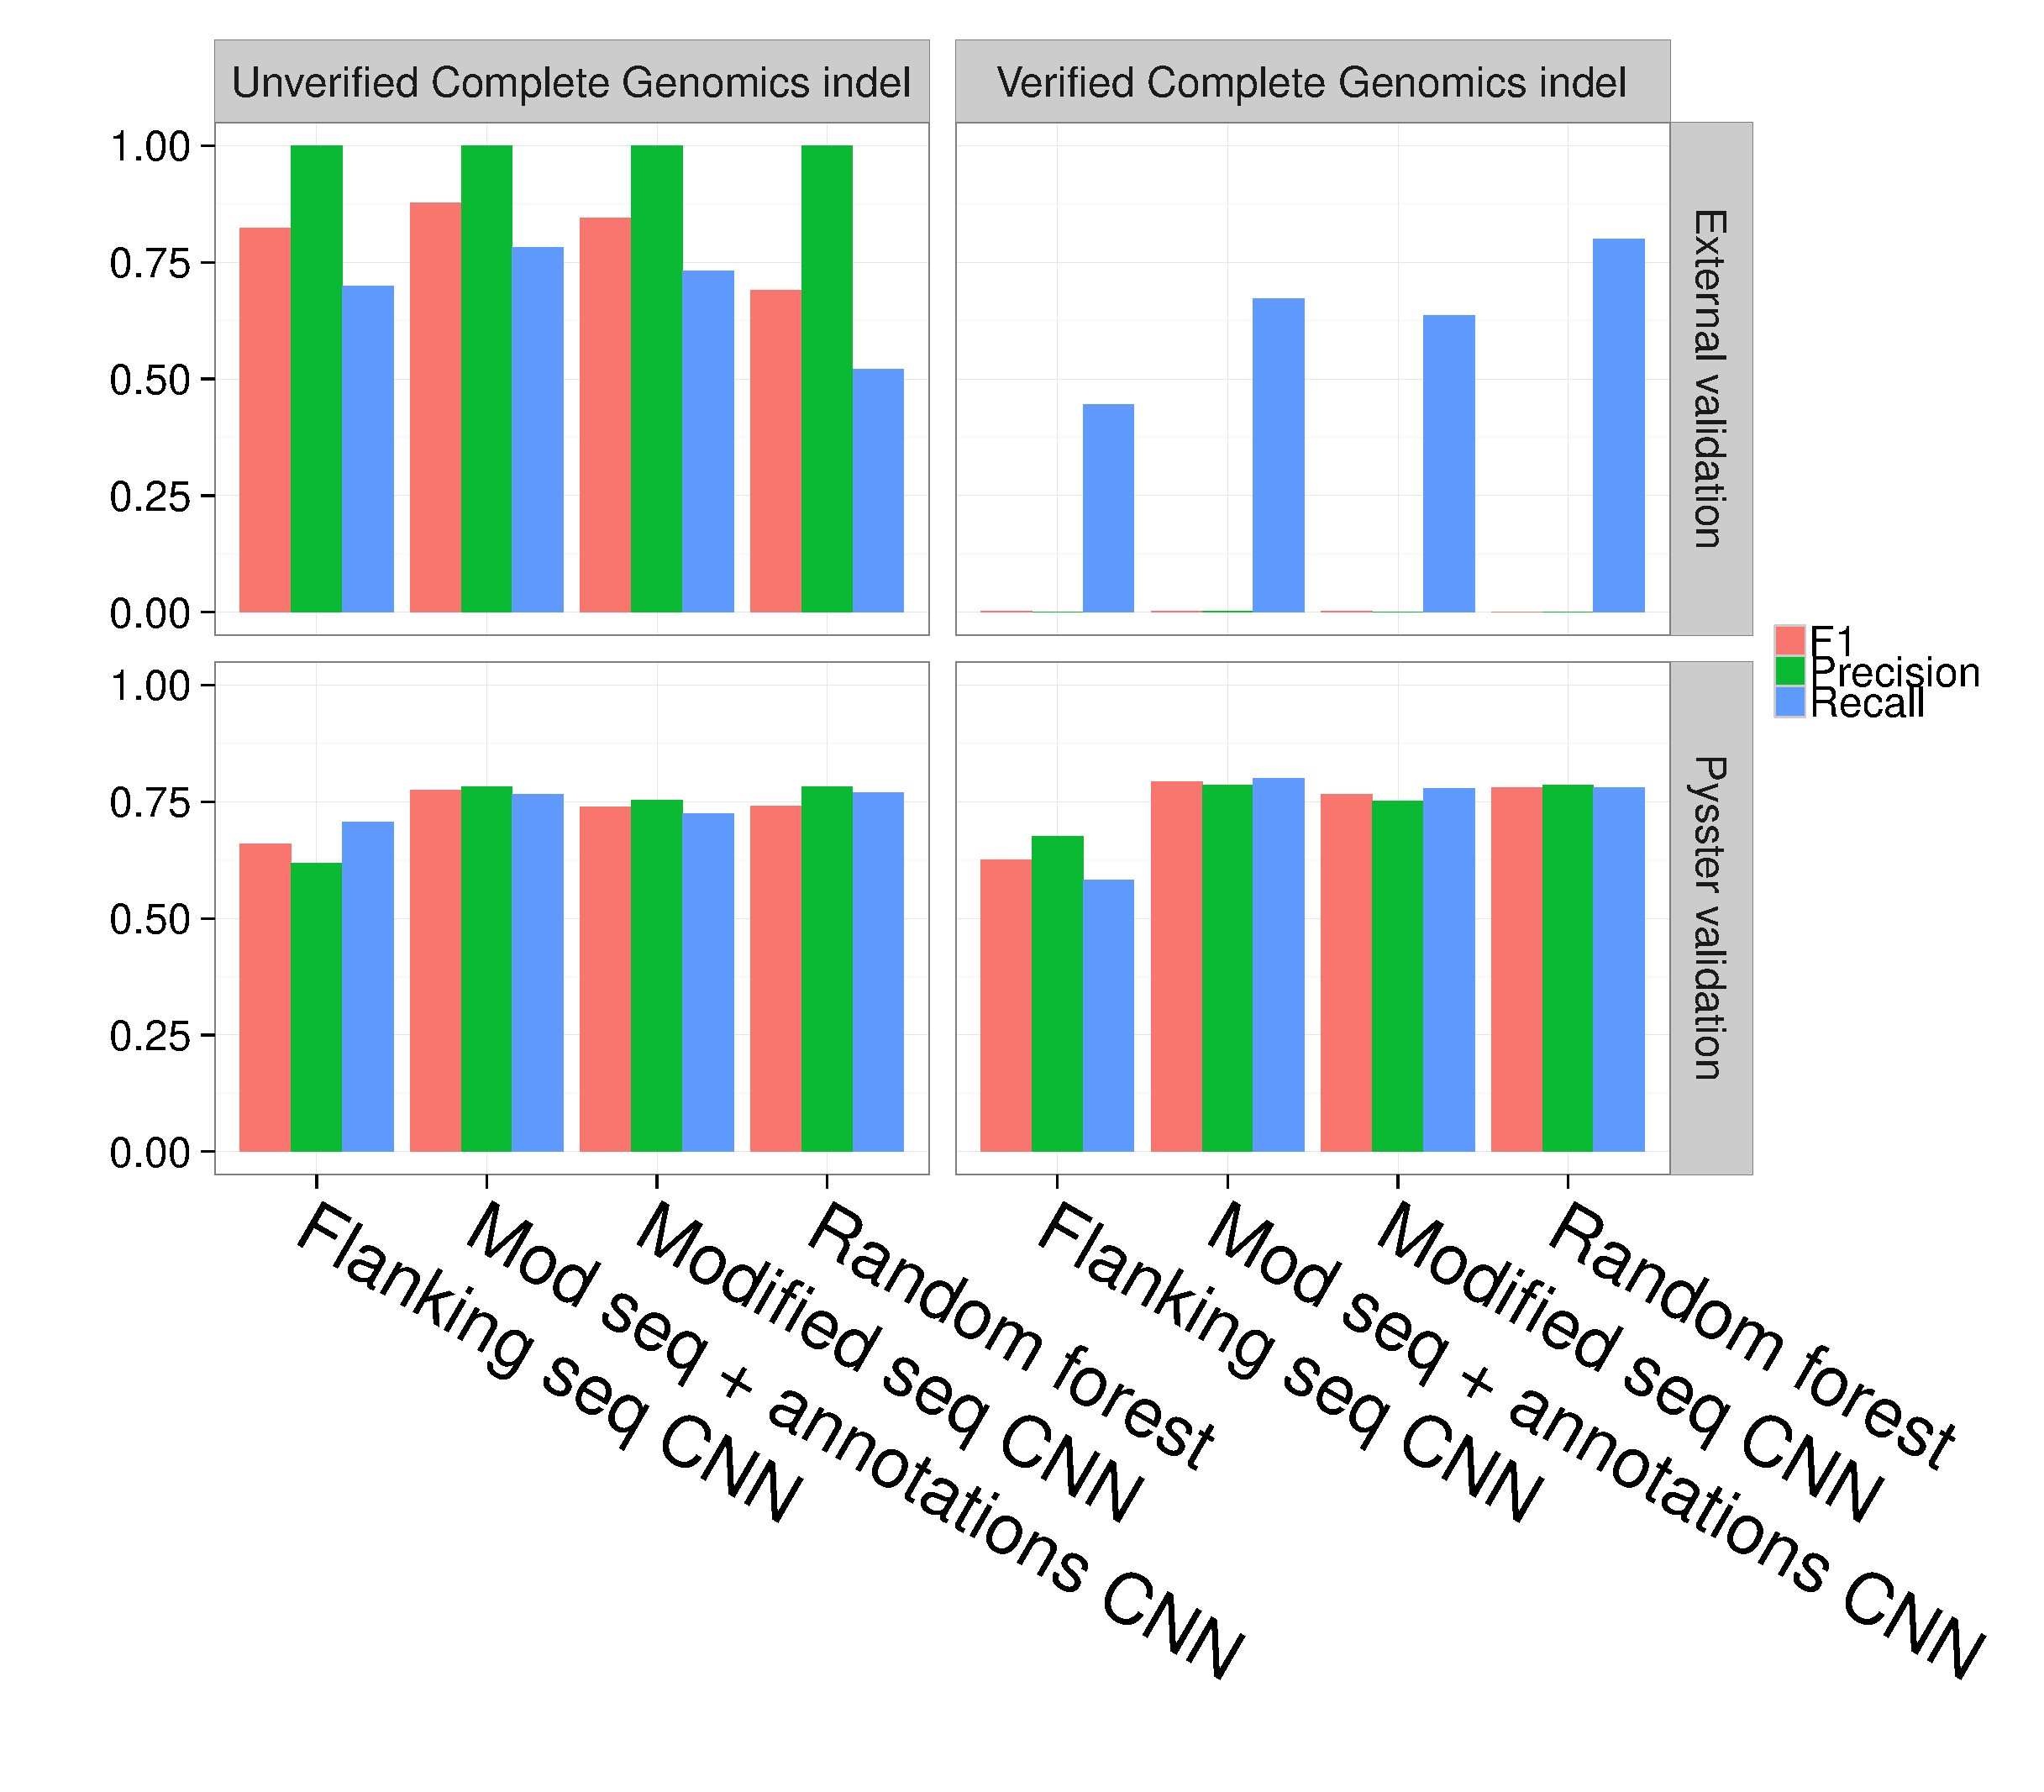
\includegraphics[width=1\linewidth]{figs/eval.eps}
\end{figure}

\begin{alertblock}{Conclusion}

\begin{itemize}
\item 93\% of Complete Genomics indels are unverified by Illumina
\item Convolutional networks from DNA sequence perform better than a random forest of annotated genomic features, and a convolutional network of sequence motif features captures most of the information provided by annotated features
\item Encoding indels into the reference sequence performs slightly better than using reference sequence context
\end{itemize}

\end{alertblock}

\end{block}

%----------------------------------------------------------------------------------------
%	REFERENCES
%----------------------------------------------------------------------------------------

\begin{block}{References}

\nocite{*} % Insert publications even if they are not cited in the poster
\small{\bibliographystyle{unsrt}
\bibliography{sample}\vspace{0.75in}}

\end{block}

\setbeamercolor{block title}{fg=red,bg=white} % Change the block title color

\setbeamercolor{block alerted title}{fg=black,bg=norange} % Change the alert block title colors
\setbeamercolor{block alerted body}{fg=black,bg=white} % Change the alert block body colors


\begin{block}{Acknowledgements}
\centering
\small{\rmfamily{Brian Ennis is supported as a DBHI student intern.}} \\

\end{block}


\begin{center}
\begin{tabular}{ccc}

\includegraphics[width=0.4\linewidth]{figs/chop.jpg} & \hfill & 
\includegraphics[width=0.4\linewidth]{figs/dbhi.png}
\end{tabular}
\end{center}

%----------------------------------------------------------------------------------------

\end{column} % End of the third column